\documentclass[]{article}
\usepackage{lmodern}
\usepackage{amssymb,amsmath}
\usepackage{ifxetex,ifluatex}
\usepackage{fixltx2e} % provides \textsubscript
\ifnum 0\ifxetex 1\fi\ifluatex 1\fi=0 % if pdftex
  \usepackage[T1]{fontenc}
  \usepackage[utf8]{inputenc}
\else % if luatex or xelatex
  \ifxetex
    \usepackage{mathspec}
  \else
    \usepackage{fontspec}
  \fi
  \defaultfontfeatures{Ligatures=TeX,Scale=MatchLowercase}
\fi
% use upquote if available, for straight quotes in verbatim environments
\IfFileExists{upquote.sty}{\usepackage{upquote}}{}
% use microtype if available
\IfFileExists{microtype.sty}{%
\usepackage{microtype}
\UseMicrotypeSet[protrusion]{basicmath} % disable protrusion for tt fonts
}{}
\usepackage[margin=1in]{geometry}
\usepackage{hyperref}
\hypersetup{unicode=true,
            pdftitle={Assignment 9},
            pdfauthor={Reid Ginoza},
            pdfborder={0 0 0},
            breaklinks=true}
\urlstyle{same}  % don't use monospace font for urls
\usepackage{color}
\usepackage{fancyvrb}
\newcommand{\VerbBar}{|}
\newcommand{\VERB}{\Verb[commandchars=\\\{\}]}
\DefineVerbatimEnvironment{Highlighting}{Verbatim}{commandchars=\\\{\}}
% Add ',fontsize=\small' for more characters per line
\usepackage{framed}
\definecolor{shadecolor}{RGB}{248,248,248}
\newenvironment{Shaded}{\begin{snugshade}}{\end{snugshade}}
\newcommand{\AlertTok}[1]{\textcolor[rgb]{0.94,0.16,0.16}{#1}}
\newcommand{\AnnotationTok}[1]{\textcolor[rgb]{0.56,0.35,0.01}{\textbf{\textit{#1}}}}
\newcommand{\AttributeTok}[1]{\textcolor[rgb]{0.77,0.63,0.00}{#1}}
\newcommand{\BaseNTok}[1]{\textcolor[rgb]{0.00,0.00,0.81}{#1}}
\newcommand{\BuiltInTok}[1]{#1}
\newcommand{\CharTok}[1]{\textcolor[rgb]{0.31,0.60,0.02}{#1}}
\newcommand{\CommentTok}[1]{\textcolor[rgb]{0.56,0.35,0.01}{\textit{#1}}}
\newcommand{\CommentVarTok}[1]{\textcolor[rgb]{0.56,0.35,0.01}{\textbf{\textit{#1}}}}
\newcommand{\ConstantTok}[1]{\textcolor[rgb]{0.00,0.00,0.00}{#1}}
\newcommand{\ControlFlowTok}[1]{\textcolor[rgb]{0.13,0.29,0.53}{\textbf{#1}}}
\newcommand{\DataTypeTok}[1]{\textcolor[rgb]{0.13,0.29,0.53}{#1}}
\newcommand{\DecValTok}[1]{\textcolor[rgb]{0.00,0.00,0.81}{#1}}
\newcommand{\DocumentationTok}[1]{\textcolor[rgb]{0.56,0.35,0.01}{\textbf{\textit{#1}}}}
\newcommand{\ErrorTok}[1]{\textcolor[rgb]{0.64,0.00,0.00}{\textbf{#1}}}
\newcommand{\ExtensionTok}[1]{#1}
\newcommand{\FloatTok}[1]{\textcolor[rgb]{0.00,0.00,0.81}{#1}}
\newcommand{\FunctionTok}[1]{\textcolor[rgb]{0.00,0.00,0.00}{#1}}
\newcommand{\ImportTok}[1]{#1}
\newcommand{\InformationTok}[1]{\textcolor[rgb]{0.56,0.35,0.01}{\textbf{\textit{#1}}}}
\newcommand{\KeywordTok}[1]{\textcolor[rgb]{0.13,0.29,0.53}{\textbf{#1}}}
\newcommand{\NormalTok}[1]{#1}
\newcommand{\OperatorTok}[1]{\textcolor[rgb]{0.81,0.36,0.00}{\textbf{#1}}}
\newcommand{\OtherTok}[1]{\textcolor[rgb]{0.56,0.35,0.01}{#1}}
\newcommand{\PreprocessorTok}[1]{\textcolor[rgb]{0.56,0.35,0.01}{\textit{#1}}}
\newcommand{\RegionMarkerTok}[1]{#1}
\newcommand{\SpecialCharTok}[1]{\textcolor[rgb]{0.00,0.00,0.00}{#1}}
\newcommand{\SpecialStringTok}[1]{\textcolor[rgb]{0.31,0.60,0.02}{#1}}
\newcommand{\StringTok}[1]{\textcolor[rgb]{0.31,0.60,0.02}{#1}}
\newcommand{\VariableTok}[1]{\textcolor[rgb]{0.00,0.00,0.00}{#1}}
\newcommand{\VerbatimStringTok}[1]{\textcolor[rgb]{0.31,0.60,0.02}{#1}}
\newcommand{\WarningTok}[1]{\textcolor[rgb]{0.56,0.35,0.01}{\textbf{\textit{#1}}}}
\usepackage{graphicx,grffile}
\makeatletter
\def\maxwidth{\ifdim\Gin@nat@width>\linewidth\linewidth\else\Gin@nat@width\fi}
\def\maxheight{\ifdim\Gin@nat@height>\textheight\textheight\else\Gin@nat@height\fi}
\makeatother
% Scale images if necessary, so that they will not overflow the page
% margins by default, and it is still possible to overwrite the defaults
% using explicit options in \includegraphics[width, height, ...]{}
\setkeys{Gin}{width=\maxwidth,height=\maxheight,keepaspectratio}
\IfFileExists{parskip.sty}{%
\usepackage{parskip}
}{% else
\setlength{\parindent}{0pt}
\setlength{\parskip}{6pt plus 2pt minus 1pt}
}
\setlength{\emergencystretch}{3em}  % prevent overfull lines
\providecommand{\tightlist}{%
  \setlength{\itemsep}{0pt}\setlength{\parskip}{0pt}}
\setcounter{secnumdepth}{0}
% Redefines (sub)paragraphs to behave more like sections
\ifx\paragraph\undefined\else
\let\oldparagraph\paragraph
\renewcommand{\paragraph}[1]{\oldparagraph{#1}\mbox{}}
\fi
\ifx\subparagraph\undefined\else
\let\oldsubparagraph\subparagraph
\renewcommand{\subparagraph}[1]{\oldsubparagraph{#1}\mbox{}}
\fi

%%% Use protect on footnotes to avoid problems with footnotes in titles
\let\rmarkdownfootnote\footnote%
\def\footnote{\protect\rmarkdownfootnote}

%%% Change title format to be more compact
\usepackage{titling}

% Create subtitle command for use in maketitle
\providecommand{\subtitle}[1]{
  \posttitle{
    \begin{center}\large#1\end{center}
    }
}

\setlength{\droptitle}{-2em}

  \title{Assignment 9}
    \pretitle{\vspace{\droptitle}\centering\huge}
  \posttitle{\par}
    \author{Reid Ginoza}
    \preauthor{\centering\large\emph}
  \postauthor{\par}
      \predate{\centering\large\emph}
  \postdate{\par}
    \date{4/12/2020}

\newcommand{\D}{\mathrm{d}}
\DeclareMathOperator*{\argmin}{arg\,min}

\begin{document}
\maketitle

\hypertarget{analytical-maximum-likelihood}{%
\section{Analytical Maximum
Likelihood}\label{analytical-maximum-likelihood}}

This is Exercise 11.1 from (Särkkä and Solin 2019). We are given the
following: \begin{equation}
x_k = \theta + r_k, \quad k=1, 2, \ldots, T,
\end{equation} where
\(r_k \sim \operatorname{N}{\left( 0, \sigma^2 \right)}\) are
independent.

\hypertarget{maximum-likelihood-estimator}{%
\subsection{Maximum Likelihood
Estimator}\label{maximum-likelihood-estimator}}

Let \(L\left(\cdot\right)\) be the likelihood and
\(l\left(\cdot\right)\) be the negative log likelihood. Then, to find
the maximum likelihood estimator
\(\theta_{\textrm{ML}} = \argmin_{\theta} L\left(\theta\right)\), we
will minimize \(l \left( \theta \right)\): \begin{align}
x_k &= \theta + r_k \sim \operatorname{N}{\left( \theta, \sigma^2 \right)}\\
\implies \operatorname{f}{\left( x_k \vert \theta\right)} &= 
\dfrac{1}{\sqrt{2 \pi \sigma^2}} \exp{\left( - \dfrac{\left( x_k - \theta \right)^2}{2 \sigma^2} \right)}\\
\implies L \left( \theta \right) &= \left( 2 \pi \sigma^2 \right)^{\frac{T}{2}} \prod_{k=1}^{T} \exp{\left( - \dfrac{\left( x_k - \theta \right)^2}{2 \sigma^2} \right)}\\
&= \left( 2 \pi \sigma^2 \right)^{\frac{T}{2}} \exp{\left( - \dfrac{1}{2 \sigma^2} \sum_{k=1}^{T} \left( x_k - \theta \right)^2 \right)}\\
\implies l\left( \theta \right) &= - \dfrac{T}{2} \log{\left( 2 \pi \sigma^2 \right)} + \dfrac{1}{2 \sigma^2} \sum_{k=1}^{T} \left( x_k - \theta \right)^2\\
\text{Now, suppose } \theta_{\textrm{ML}}\text{ solves the following,} \quad \dfrac{\mathrm{d}l}{\mathrm{d}\theta} &= 0\\
&= - \dfrac{1}{\sigma^2} \sum_{k=1}^{T} \left( x_k - \theta_{\textrm{ML}} \right)\\
\implies 0 &= \sum_{k=1}^{T} \left( x_k - \theta_{\textrm{ML}} \right)\\
\implies \theta_{\textrm{ML}} &= \dfrac{1}{T} \sum_{k=1}^{T} x_k = \bar{x}
\end{align}

\hypertarget{numerical-maximum-likelihood}{%
\section{Numerical Maximum
Likelihood}\label{numerical-maximum-likelihood}}

\begin{Shaded}
\begin{Highlighting}[]
\ImportTok{import}\NormalTok{ numpy }\ImportTok{as}\NormalTok{ np}
\ImportTok{from}\NormalTok{ matplotlib }\ImportTok{import}\NormalTok{ pyplot }\ImportTok{as}\NormalTok{ plt}
\ImportTok{from}\NormalTok{ scipy.optimize }\ImportTok{import}\NormalTok{ minimize_scalar}
\ImportTok{from}\NormalTok{ scipy.stats }\ImportTok{import}\NormalTok{ norm}


\CommentTok{# -- Plotting Tools --}
\KeywordTok{def}\NormalTok{ low_buff(y_values):}
\NormalTok{    span }\OperatorTok{=}\NormalTok{ y_values.}\BuiltInTok{max}\NormalTok{() }\OperatorTok{-}\NormalTok{ y_values.}\BuiltInTok{min}\NormalTok{()}
    \ControlFlowTok{return}\NormalTok{ y_values.}\BuiltInTok{min}\NormalTok{() }\OperatorTok{-} \FloatTok{0.1} \OperatorTok{*}\NormalTok{ span}


\CommentTok{# -- True Distribution --}
\NormalTok{THETA }\OperatorTok{=} \DecValTok{1}
\NormalTok{SIGMA }\OperatorTok{=} \DecValTok{1}

\CommentTok{# -- Samples}
\NormalTok{T }\OperatorTok{=} \DecValTok{1000}

\NormalTok{r }\OperatorTok{=}\NormalTok{ np.random.normal(scale}\OperatorTok{=}\NormalTok{SIGMA, size}\OperatorTok{=}\NormalTok{(T,))}
\NormalTok{sample }\OperatorTok{=}\NormalTok{ THETA }\OperatorTok{+}\NormalTok{ r}
\BuiltInTok{print}\NormalTok{(sample.mean())}
\end{Highlighting}
\end{Shaded}

\begin{verbatim}
## 1.0138583286773388
\end{verbatim}

\begin{Shaded}
\begin{Highlighting}[]
\KeywordTok{def}\NormalTok{ neg_log_llh(theta, sample, T, sigma):}
    \ControlFlowTok{return} \OperatorTok{-}\NormalTok{ T}\OperatorTok{/}\DecValTok{2} \OperatorTok{*}\NormalTok{ np.log(}\DecValTok{2} \OperatorTok{*}\NormalTok{ np.pi }\OperatorTok{*}\NormalTok{ sigma}\OperatorTok{**}\DecValTok{2}\NormalTok{) }\OperatorTok{+} \DecValTok{1} \OperatorTok{/}\NormalTok{ (}\DecValTok{2} \OperatorTok{*}\NormalTok{ sigma) }\OperatorTok{*}\NormalTok{ ((sample }\OperatorTok{-}\NormalTok{ theta)}\OperatorTok{**}\DecValTok{2}\NormalTok{).}\BuiltInTok{sum}\NormalTok{()}


\KeywordTok{def}\NormalTok{ nll_vec(theta_plot, sample, T, sigma):}
    \ControlFlowTok{return}\NormalTok{ np.array([neg_log_llh(theta, sample, T, sigma) }\ControlFlowTok{for}\NormalTok{ theta }\KeywordTok{in}\NormalTok{ theta_plot])}


\NormalTok{theta_plot }\OperatorTok{=}\NormalTok{ np.linspace(}\DecValTok{0}\NormalTok{, }\DecValTok{3}\NormalTok{, }\DecValTok{1000}\NormalTok{)}
\NormalTok{likelihood_plot }\OperatorTok{=}\NormalTok{ nll_vec(theta_plot, sample, T, SIGMA)}
\NormalTok{estimator_result }\OperatorTok{=}\NormalTok{ minimize_scalar(neg_log_llh, args}\OperatorTok{=}\NormalTok{(sample, T, SIGMA))}

\NormalTok{fig, ax }\OperatorTok{=}\NormalTok{ plt.subplots()}
\NormalTok{ax.plot(theta_plot, likelihood_plot,}
\NormalTok{        label}\OperatorTok{=}\StringTok{'Likelihood'}\NormalTok{)}
\NormalTok{ax.vlines(x}\OperatorTok{=}\NormalTok{THETA, ymin}\OperatorTok{=}\NormalTok{low_buff(likelihood_plot), ymax}\OperatorTok{=}\NormalTok{likelihood_plot.}\BuiltInTok{max}\NormalTok{(),}
\NormalTok{          label}\OperatorTok{=}\StringTok{'True Parameter'}\NormalTok{)}
\NormalTok{ax.plot(sample.mean(), neg_log_llh(sample.mean(), sample, T, SIGMA), }\StringTok{'o'}\NormalTok{,}
\NormalTok{          label}\OperatorTok{=}\StringTok{'ML Estimator}\CharTok{\textbackslash{}n}\StringTok{'} \OperatorTok{+} \VerbatimStringTok{r'$\textbackslash{}theta_\{\textbackslash{}mathrm}\SpecialCharTok{\{ML\}}\VerbatimStringTok{\} = '} \OperatorTok{+} \BuiltInTok{str}\NormalTok{(}\BuiltInTok{round}\NormalTok{(sample.mean(), }\DecValTok{3}\NormalTok{)) }\OperatorTok{+} \StringTok{'$'}\NormalTok{)}
\CommentTok{# ax.plot(estimator_result.x, estimator_result.fun, 'o',}
\CommentTok{#         label=f'Numerical Minimization: \{round(estimator_result.x, 3)\},'}
\CommentTok{#               f' \{round(estimator_result.fun, 3)\}')}
\NormalTok{ax.set_xlabel(}\VerbatimStringTok{r'$\textbackslash{}theta$'}\NormalTok{)}
\NormalTok{ax.set_ylabel(}\StringTok{'Likelihood '} \OperatorTok{+} \VerbatimStringTok{r'$L(\textbackslash{}theta)$'}\NormalTok{)}
\NormalTok{ax.set_title(}\StringTok{'Likelihood Function'}\NormalTok{)}
\NormalTok{ax.legend()}
\NormalTok{plt.show()}
\end{Highlighting}
\end{Shaded}

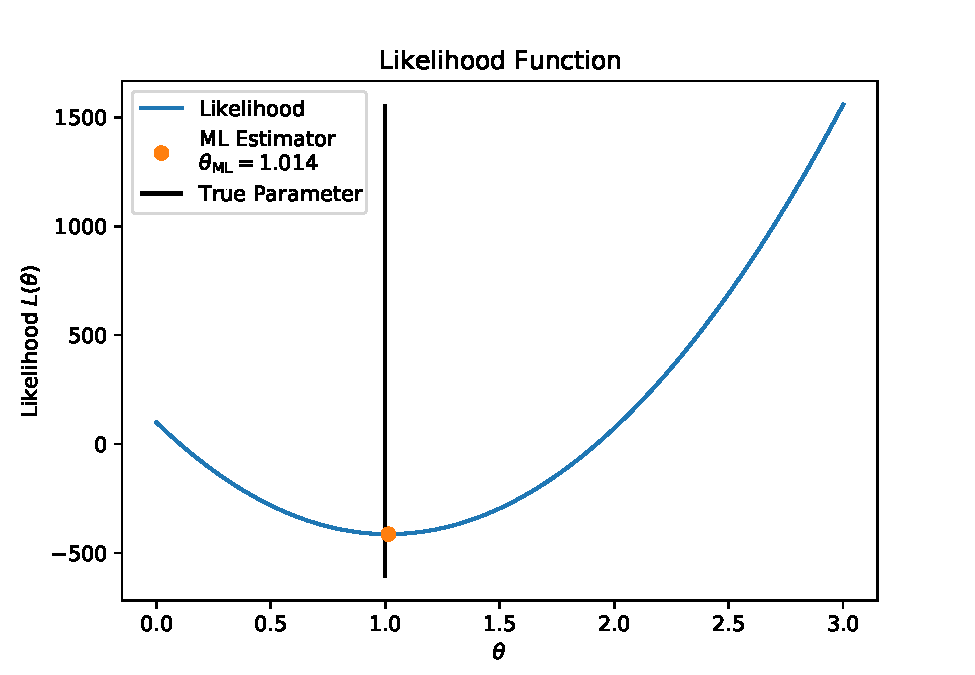
\includegraphics{/Users/macowner/Documents/Stochastic_Calculus/Hmwk_09/hmwk_09_files/figure-latex/ml1-1.pdf}

\hypertarget{analytical-maximum-a-posteriori}{%
\section{Analytical Maximum A
Posteriori}\label{analytical-maximum-a-posteriori}}

This is Exercise 11.2 from (Särkkä and Solin 2019). Since this is not a
nonlinear SDE, we can use the following to determine the posterior
probability distribution: \begin{align}
p\left(\theta | x\left(t_1\right), \ldots, x\left(t_T\right)\right) &\sim
  p\left(\theta\right) \exp{\left( -l\left(\theta\right)\right)} = \exp{\left( -l_p\left( \theta \right) \right)}\\
&= \left[
    \dfrac{1}{\sqrt{2\pi\lambda^2}} \exp{\left(- \dfrac{\theta^2}{2\lambda^2}\right)}
\right]
\left[
    \exp{\left(
        \dfrac{T}{2} \log{\left( 2 \pi \sigma^2 \right)} - \dfrac{1}{2 \sigma^2} \sum_{k=1}^{T} \left( x_k - \theta \right)^2
    \right)}
\right]\\
&= \left( 2 \pi \lambda^2 \right)^\frac{1}{2}
    \exp{ \left(
        - \dfrac{\theta^2}{2\lambda^2} + \dfrac{T}{2} \log{\left( 2 \pi \sigma^2 \right)} - \dfrac{1}{2 \sigma^2} \sum_{k=1}^{T} \left( x_k - \theta \right)^2
    \right) }
\end{align}

and to find the maximimum a posteriori estimate,
\(\theta_{\textrm{MAP}} = \argmin_\theta p\left(\theta | x\left(t_1\right), \ldots, x\left(t_T\right)\right)\),
we minimize the negative logarithm of the posterior distribution, which
we'll call \(A\). \begin{align}
A &=
- \log{\left(
\left( 2 \pi \lambda^2 \right)^\frac{1}{2}
    \exp{ \left(
        - \dfrac{\theta^2}{2\lambda^2} + \dfrac{T}{2} \log{\left( 2 \pi \sigma^2 \right)} - \dfrac{1}{2 \sigma^2} \sum_{k=1}^{T} \left( x_k - \theta \right)^2
    \right) }
\right)}\\
&= - \dfrac{1}{2}\log{\left( 2 \pi \lambda^2 \right)}
+ \dfrac{\theta^2}{2\lambda^2} - \dfrac{T}{2} \log{\left( 2 \pi \sigma^2 \right)} + \dfrac{1}{2 \sigma^2} \sum_{k=1}^{T} \left( x_k - \theta \right)^2\\
&= - \dfrac{1}{2}\log{\left( 2 \pi \lambda^2 \right)}
+ \dfrac{\theta^2}{2\lambda^2} - \dfrac{T}{2} \log{\left( 2 \pi \sigma^2 \right)}
  + \dfrac{1}{2 \sigma^2} \sum_{k=1}^{T} x_k^2
  -2 \theta \dfrac{1}{2 \sigma^2} \sum_{k=1}^{T} x_k
  + \dfrac{1}{2 \sigma^2} T \theta^2\\
&= \left[ \dfrac{1}{2\lambda^2} + \dfrac{T}{2\sigma^2} \right]\theta^2
- \left[\dfrac{1}{\sigma^2} \sum_{k=1}^T x_k \right] \theta
+ \left[ \dfrac{1}{2 \sigma^2} \sum_{k=1}^{T} x_k^2
- \dfrac{1}{2}\log{\left( 2 \pi \lambda^2 \right)}
\right]
\end{align}

Since \(A\) is quadratic in \(\theta\), we can use the familiar formula
for the minimum. \begin{align}
\theta_{\mathrm{MAP}} &= \dfrac{\dfrac{1}{\sigma^2} \sum_{k=1}^T x_k}{\dfrac{1}{\lambda^2} + \dfrac{T}{\sigma^2}}\\
&= \dfrac{\dfrac{1}{\sigma^2} \sum_{k=1}^T x_k}
{\dfrac{T\lambda^2 + \sigma^2}{\lambda^2\sigma^2}}\\
&= \dfrac{\lambda^2}{T\lambda^2 + \sigma^2} \sum_{k=1}^T x_k\\
&= \dfrac{1}{T + \dfrac{\sigma^2}{\lambda^2}} \sum_{k=1}^T x_k
\end{align}

\hypertarget{numerical-map-estimator}{%
\section{Numerical MAP Estimator}\label{numerical-map-estimator}}

\begin{Shaded}
\begin{Highlighting}[]
\CommentTok{# -- Prior --}
\NormalTok{LAMBDA }\OperatorTok{=} \DecValTok{2}


\KeywordTok{def}\NormalTok{ prior(theta, lamb):}
    \ControlFlowTok{return} \DecValTok{1} \OperatorTok{/}\NormalTok{ np.sqrt(}\DecValTok{2} \OperatorTok{*}\NormalTok{ np.pi }\OperatorTok{*}\NormalTok{ lamb}\OperatorTok{**}\DecValTok{2}\NormalTok{) }\OperatorTok{*}\NormalTok{ np.exp(}\OperatorTok{-}\NormalTok{ theta}\OperatorTok{**}\DecValTok{2} \OperatorTok{/}\NormalTok{ (}\DecValTok{2} \OperatorTok{*}\NormalTok{ lamb}\OperatorTok{**}\DecValTok{2}\NormalTok{))}


\KeywordTok{def}\NormalTok{ posterior(theta, lamb, sigma, sample):}
    \CommentTok{""" f1 * exp(f2 + f3 + f4) """}
\NormalTok{    f1 }\OperatorTok{=}\NormalTok{ np.sqrt(}\DecValTok{2} \OperatorTok{*}\NormalTok{ np.pi }\OperatorTok{*}\NormalTok{ lamb}\OperatorTok{**}\DecValTok{2}\NormalTok{)}
\NormalTok{    f2 }\OperatorTok{=} \OperatorTok{-}\NormalTok{ theta}\OperatorTok{**}\DecValTok{2} \OperatorTok{/}\NormalTok{ (}\DecValTok{2} \OperatorTok{*}\NormalTok{ lamb}\OperatorTok{**}\DecValTok{2}\NormalTok{)}
\NormalTok{    f3 }\OperatorTok{=}\NormalTok{ sample.size }\OperatorTok{/} \DecValTok{2} \OperatorTok{*}\NormalTok{ np.log(}\DecValTok{2} \OperatorTok{*}\NormalTok{ np.pi }\OperatorTok{*}\NormalTok{ sigma}\OperatorTok{**}\DecValTok{2}\NormalTok{)}
\NormalTok{    f4 }\OperatorTok{=} \OperatorTok{-} \DecValTok{1} \OperatorTok{/}\NormalTok{ (}\DecValTok{2} \OperatorTok{*}\NormalTok{ sigma}\OperatorTok{**}\DecValTok{2}\NormalTok{ ) }\OperatorTok{*}\NormalTok{ np.}\BuiltInTok{sum}\NormalTok{((sample }\OperatorTok{-}\NormalTok{ theta)}\OperatorTok{**}\DecValTok{2}\NormalTok{)}
    \ControlFlowTok{return}\NormalTok{ f1 }\OperatorTok{*}\NormalTok{ np.exp(f2 }\OperatorTok{+}\NormalTok{ f3 }\OperatorTok{+}\NormalTok{ f4)}


\KeywordTok{def}\NormalTok{ map_estimate(T, sigma, lamb, sample):}
    \CommentTok{""" Uses analytical formula found by minimizing the}
\CommentTok{    un-normalized negative log of the posterior """}
    \ControlFlowTok{return} \DecValTok{1} \OperatorTok{/}\NormalTok{ (T }\OperatorTok{+}\NormalTok{ sigma}\OperatorTok{**}\DecValTok{2}\OperatorTok{/}\NormalTok{lamb}\OperatorTok{**}\DecValTok{2}\NormalTok{) }\OperatorTok{*}\NormalTok{ sample.}\BuiltInTok{sum}\NormalTok{()}


\KeywordTok{def}\NormalTok{ this_neg_posterior(theta):}
    \CommentTok{""" dependent on current samples}
\CommentTok{    convenience function for optimizer of the posterior}
\CommentTok{    without mixing arrays (i.e. sample size vs attempted theta) """}
    \ControlFlowTok{return} \DecValTok{-1} \OperatorTok{*}\NormalTok{ posterior(theta, LAMBDA, SIGMA, sample)}


\CommentTok{# Find Estimators}
\NormalTok{num_map_estimate }\OperatorTok{=}\NormalTok{ minimize_scalar(this_neg_posterior)}
\NormalTok{theta_map }\OperatorTok{=}\NormalTok{ map_estimate(T, SIGMA, LAMBDA, sample)}

\CommentTok{# plotting}
\NormalTok{theta_plot }\OperatorTok{=}\NormalTok{ np.linspace(}\OperatorTok{-}\DecValTok{5}\NormalTok{, }\DecValTok{5}\NormalTok{, }\DecValTok{5000}\NormalTok{)}
\NormalTok{prior_plot }\OperatorTok{=}\NormalTok{ prior(theta_plot, LAMBDA)}
\NormalTok{posterior_plot }\OperatorTok{=}\NormalTok{ np.array([posterior(th, LAMBDA, SIGMA, sample) }\ControlFlowTok{for}\NormalTok{ th }\KeywordTok{in}\NormalTok{ theta_plot])}

\NormalTok{fig2, axes2 }\OperatorTok{=}\NormalTok{ plt.subplots(nrows}\OperatorTok{=}\DecValTok{2}\NormalTok{)}
\CommentTok{# prior plot}
\NormalTok{axes2[}\DecValTok{0}\NormalTok{].plot(theta_plot, prior_plot, label}\OperatorTok{=}\StringTok{'Prior'}\NormalTok{)}
\NormalTok{axes2[}\DecValTok{0}\NormalTok{].vlines(x}\OperatorTok{=}\NormalTok{THETA, ymin}\OperatorTok{=}\NormalTok{low_buff(prior_plot), ymax}\OperatorTok{=}\NormalTok{prior_plot.}\BuiltInTok{max}\NormalTok{(),}
\NormalTok{          label}\OperatorTok{=}\StringTok{'True Parameter'}\NormalTok{)}
\NormalTok{axes2[}\DecValTok{0}\NormalTok{].set_title(}\StringTok{'Prior Distribution'}\NormalTok{)}
\NormalTok{axes2[}\DecValTok{0}\NormalTok{].legend()}

\CommentTok{# posterior plot}
\CommentTok{# Doesn't make sense to show prior since posterior is un-normalized}
\CommentTok{# axes2[1].plot(theta_plot, prior_plot, label='Prior', ls='dashed', alpha=0.8)}
\NormalTok{axes2[}\DecValTok{1}\NormalTok{].plot(theta_plot, posterior_plot, label}\OperatorTok{=}\StringTok{'Un-normalized Posterior'}\NormalTok{)}
\NormalTok{axes2[}\DecValTok{1}\NormalTok{].vlines(x}\OperatorTok{=}\NormalTok{THETA, ymin}\OperatorTok{=}\NormalTok{low_buff(posterior_plot), ymax}\OperatorTok{=}\NormalTok{posterior_plot.}\BuiltInTok{max}\NormalTok{(),}
\NormalTok{          label}\OperatorTok{=}\SpecialStringTok{f'True Parameter: }\SpecialCharTok{\{}\NormalTok{THETA}\SpecialCharTok{\}}\SpecialStringTok{'}\NormalTok{)}
\NormalTok{axes2[}\DecValTok{1}\NormalTok{].vlines(x}\OperatorTok{=}\NormalTok{theta_map, ymin}\OperatorTok{=}\NormalTok{low_buff(posterior_plot), ymax}\OperatorTok{=}\NormalTok{posterior_plot.}\BuiltInTok{max}\NormalTok{(),}
\NormalTok{          colors}\OperatorTok{=}\StringTok{'m'}\NormalTok{, label}\OperatorTok{=}\SpecialStringTok{f'MAP Estimator: }\SpecialCharTok{\{}\BuiltInTok{round}\NormalTok{(theta_map, }\DecValTok{3}\NormalTok{)}\SpecialCharTok{\}}\SpecialStringTok{'}\NormalTok{)}
\NormalTok{axes2[}\DecValTok{1}\NormalTok{].vlines(x}\OperatorTok{=}\NormalTok{num_map_estimate.x, ymin}\OperatorTok{=}\NormalTok{low_buff(posterior_plot), ymax}\OperatorTok{=}\NormalTok{posterior_plot.}\BuiltInTok{max}\NormalTok{(),}
\NormalTok{          colors}\OperatorTok{=}\StringTok{'r'}\NormalTok{, label}\OperatorTok{=}\SpecialStringTok{f'Numerical MAP}\CharTok{\textbackslash{}n}\SpecialStringTok{Estimator: }\SpecialCharTok{\{}\BuiltInTok{round}\NormalTok{(num_map_estimate.x, }\DecValTok{3}\NormalTok{)}\SpecialCharTok{\}}\SpecialStringTok{'}\NormalTok{)}
\NormalTok{axes2[}\DecValTok{1}\NormalTok{].set_xlim(left}\OperatorTok{=}\DecValTok{0}\NormalTok{, right}\OperatorTok{=}\DecValTok{2}\NormalTok{)}
\end{Highlighting}
\end{Shaded}

\begin{verbatim}
## (0.0, 2.0)
\end{verbatim}

\begin{Shaded}
\begin{Highlighting}[]
\NormalTok{axes2[}\DecValTok{1}\NormalTok{].set_title(}\StringTok{'Posterior Distribution'}\NormalTok{)}
\NormalTok{axes2[}\DecValTok{1}\NormalTok{].legend()}
\NormalTok{fig2.tight_layout()}
\NormalTok{plt.show()}
\end{Highlighting}
\end{Shaded}

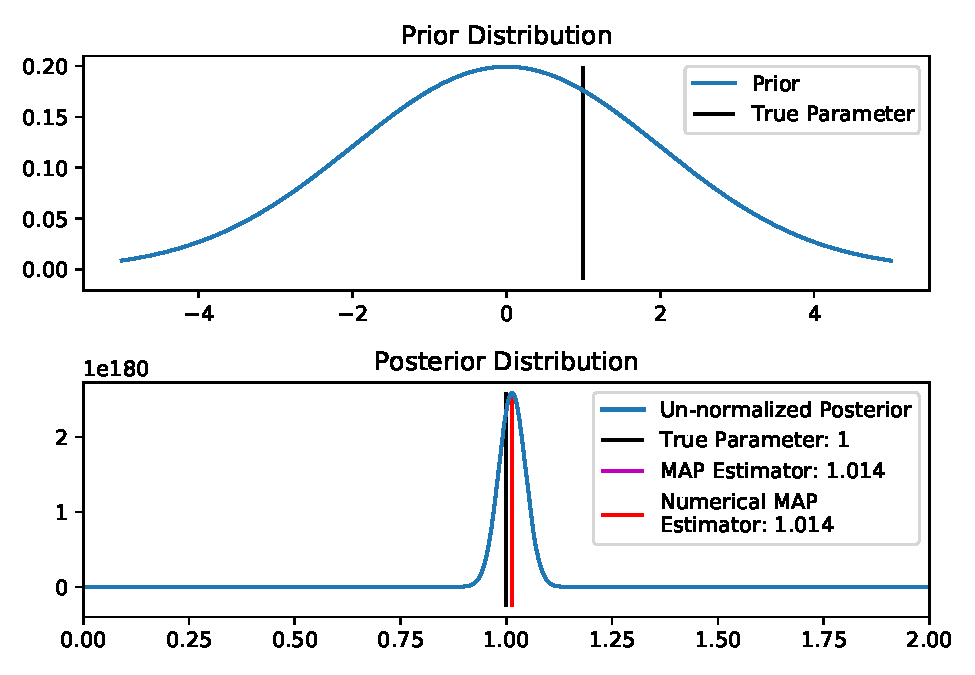
\includegraphics{/Users/macowner/Documents/Stochastic_Calculus/Hmwk_09/hmwk_09_files/figure-latex/MAP estimator-1.pdf}

\hypertarget{metropolis-hastings-algorithm}{%
\section{Metropolis-Hastings
Algorithm}\label{metropolis-hastings-algorithm}}

This is Exercise 11.3 from (Särkkä and Solin 2019). This is strictly a
coding exercise, using the Metropolis-Hastings algorithm to approximate
the posterior distribution.

\begin{Shaded}
\begin{Highlighting}[]
\CommentTok{# Functions for M-H Algorithm}
\KeywordTok{def}\NormalTok{ sample_proposal(cur_theta, gamma):}
    \ControlFlowTok{return}\NormalTok{ np.random.normal(loc}\OperatorTok{=}\NormalTok{cur_theta, scale}\OperatorTok{=}\NormalTok{gamma)}


\KeywordTok{def}\NormalTok{ proposal_probability(prop_theta, loc, gamma):}
    \ControlFlowTok{return}\NormalTok{ norm(loc}\OperatorTok{=}\NormalTok{loc, scale}\OperatorTok{=}\NormalTok{gamma).pdf(prop_theta)}


\KeywordTok{def}\NormalTok{ l_p(theta, lamb, sigma, sample):}
    \CommentTok{""" Notes on derivation}
\CommentTok{    l(th) is the negative log-likelihood}
\CommentTok{    p(th) is the prior distribution}

\CommentTok{    l_p = l(th) - log(p(th))}
\CommentTok{        = - log( p(th) * exp(-l(th) )}

\CommentTok{    written in the form f1*theta**2 + f2 * theta + f3 + f4}
\CommentTok{    """}
\NormalTok{    T }\OperatorTok{=}\NormalTok{ sample.size}
\NormalTok{    f1 }\OperatorTok{=} \DecValTok{1} \OperatorTok{/}\NormalTok{ (}\DecValTok{2} \OperatorTok{*}\NormalTok{ lamb}\OperatorTok{**}\DecValTok{2}\NormalTok{) }\OperatorTok{+}\NormalTok{ T }\OperatorTok{/}\NormalTok{ (}\DecValTok{2} \OperatorTok{*}\NormalTok{ sigma}\OperatorTok{**}\DecValTok{2}\NormalTok{)}
\NormalTok{    f2 }\OperatorTok{=} \OperatorTok{-} \DecValTok{1} \OperatorTok{/}\NormalTok{ sigma}\OperatorTok{**}\DecValTok{2} \OperatorTok{*}\NormalTok{ (sample.}\BuiltInTok{sum}\NormalTok{())}
\NormalTok{    f3 }\OperatorTok{=} \DecValTok{1} \OperatorTok{/}\NormalTok{ (}\DecValTok{2} \OperatorTok{*}\NormalTok{ sigma}\OperatorTok{**}\DecValTok{2}\NormalTok{) }\OperatorTok{*}\NormalTok{ np.}\BuiltInTok{sum}\NormalTok{((sample}\OperatorTok{**}\DecValTok{2}\NormalTok{))}
\NormalTok{    f4 }\OperatorTok{=} \OperatorTok{-} \DecValTok{1}\OperatorTok{/}\DecValTok{2} \OperatorTok{*}\NormalTok{ np.log(}\DecValTok{2} \OperatorTok{*}\NormalTok{ np.pi }\OperatorTok{*}\NormalTok{ lamb}\OperatorTok{**}\DecValTok{2}\NormalTok{)}
    \ControlFlowTok{return}\NormalTok{ f1 }\OperatorTok{*}\NormalTok{ theta}\OperatorTok{**}\DecValTok{2} \OperatorTok{+}\NormalTok{ f2 }\OperatorTok{*}\NormalTok{ theta }\OperatorTok{+}\NormalTok{ f3 }\OperatorTok{+}\NormalTok{ f4}


\KeywordTok{def}\NormalTok{ acceptance_probability(cur_theta, prop_theta, lamb, sigma, sample, gamma):}
\NormalTok{    ratio_1 }\OperatorTok{=}\NormalTok{ np.exp(l_p(cur_theta, lamb, sigma, sample)}
                     \OperatorTok{-}\NormalTok{ l_p(prop_theta, lamb, sigma, sample))}
\NormalTok{    ratio_2 }\OperatorTok{=}\NormalTok{ (proposal_probability(cur_theta, prop_theta, gamma)}
               \OperatorTok{/}\NormalTok{ proposal_probability(prop_theta, cur_theta, gamma))}
    \ControlFlowTok{return} \BuiltInTok{min}\NormalTok{(}\DecValTok{1}\NormalTok{, ratio_1 }\OperatorTok{*}\NormalTok{ ratio_2)}


\KeywordTok{def}\NormalTok{ metropolis_hastings(theta_0, gamma, lamb, sigma, sample, num_steps):}
\NormalTok{    mcmc_sampling }\OperatorTok{=}\NormalTok{ [theta_0]}
\NormalTok{    cur_theta }\OperatorTok{=}\NormalTok{ theta_0}
\NormalTok{    accept_count }\OperatorTok{=} \DecValTok{0}
    \ControlFlowTok{for}\NormalTok{ _ }\KeywordTok{in} \BuiltInTok{range}\NormalTok{(num_steps):}
\NormalTok{        prop_theta }\OperatorTok{=}\NormalTok{ sample_proposal(cur_theta, gamma)}
\NormalTok{        alpha }\OperatorTok{=}\NormalTok{ acceptance_probability(}
\NormalTok{            cur_theta, prop_theta,lamb, sigma, sample, gamma}
\NormalTok{        )}
\NormalTok{        u }\OperatorTok{=}\NormalTok{ np.random.uniform()}
        \ControlFlowTok{if}\NormalTok{ u }\OperatorTok{<}\NormalTok{ alpha:  }\CommentTok{# accept}
\NormalTok{            mcmc_sampling.append(prop_theta)}
\NormalTok{            cur_theta }\OperatorTok{=}\NormalTok{ prop_theta}
\NormalTok{            accept_count }\OperatorTok{+=} \DecValTok{1}
        \ControlFlowTok{else}\NormalTok{:}
\NormalTok{            mcmc_sampling.append(cur_theta)}
\NormalTok{    acceptance_rate }\OperatorTok{=}\NormalTok{ accept_count }\OperatorTok{/}\NormalTok{ num_steps}
    \BuiltInTok{print}\NormalTok{(}\SpecialStringTok{f'Acceptance Probability: }\SpecialCharTok{\{}\NormalTok{acceptance_rate}\SpecialCharTok{\}}\SpecialStringTok{'}\NormalTok{)}
    \ControlFlowTok{return}\NormalTok{ mcmc_sampling, acceptance_rate}


\CommentTok{# Metropolis-Hastings Values}
\NormalTok{MCMC_TRIALS }\OperatorTok{=} \DecValTok{10000}
\NormalTok{THETA_0 }\OperatorTok{=} \DecValTok{0}
\NormalTok{GAMMA }\OperatorTok{=} \FloatTok{.15}

\NormalTok{mh_sampling, acceptance_rate }\OperatorTok{=}\NormalTok{ metropolis_hastings(}
\NormalTok{    THETA_0, GAMMA, LAMBDA, SIGMA, sample, MCMC_TRIALS}
\NormalTok{)}

\CommentTok{# construct analytical posterior normalized:}
\end{Highlighting}
\end{Shaded}

\begin{verbatim}
## Acceptance Probability: 0.2531
\end{verbatim}

\begin{Shaded}
\begin{Highlighting}[]
\NormalTok{mh_theta_plot }\OperatorTok{=}\NormalTok{ np.linspace(}
\NormalTok{    np.}\BuiltInTok{min}\NormalTok{(mh_sampling),}
\NormalTok{    np.}\BuiltInTok{max}\NormalTok{(mh_sampling),}
    \DecValTok{1000}\NormalTok{,}
\NormalTok{)}
\NormalTok{mh_analytical_post }\OperatorTok{=}\NormalTok{ np.array([posterior(th, LAMBDA, SIGMA, sample) }\ControlFlowTok{for}\NormalTok{ th }\KeywordTok{in}\NormalTok{ mh_theta_plot])}
\NormalTok{tmp_hist }\OperatorTok{=}\NormalTok{ np.histogram(mh_sampling, }\StringTok{'auto'}\NormalTok{)}
\NormalTok{peak }\OperatorTok{=}\NormalTok{ tmp_hist[}\DecValTok{0}\NormalTok{].}\BuiltInTok{max}\NormalTok{()}
\KeywordTok{del}\NormalTok{ tmp_hist}
\NormalTok{mh_analytical_post }\OperatorTok{*=}\NormalTok{ peak }\OperatorTok{/}\NormalTok{ mh_analytical_post.}\BuiltInTok{max}\NormalTok{()}

\CommentTok{# Plot mh_sampling over time}
\NormalTok{mh_fig, mh_axes }\OperatorTok{=}\NormalTok{ plt.subplots(nrows}\OperatorTok{=}\DecValTok{2}\NormalTok{)}
\NormalTok{mh_axes[}\DecValTok{0}\NormalTok{].plot(mh_sampling)}
\NormalTok{mh_axes[}\DecValTok{0}\NormalTok{].set_xlabel(}\StringTok{'Iteration'}\NormalTok{)}
\NormalTok{mh_axes[}\DecValTok{0}\NormalTok{].set_ylabel(}\VerbatimStringTok{r'$\textbackslash{}theta$'}\NormalTok{)}
\NormalTok{mh_axes[}\DecValTok{0}\NormalTok{].set_title(}\SpecialStringTok{f'Sampling History}\CharTok{\textbackslash{}n}\SpecialStringTok{Acceptance Rate: }\SpecialCharTok{\{}\BuiltInTok{round}\NormalTok{(acceptance_rate, }\DecValTok{3}\NormalTok{)}\SpecialCharTok{\}}\SpecialStringTok{'}\NormalTok{)}

\CommentTok{# Plot distribution}
\NormalTok{_ }\OperatorTok{=}\NormalTok{ mh_axes[}\DecValTok{1}\NormalTok{].hist(mh_sampling, bins}\OperatorTok{=}\StringTok{'auto'}\NormalTok{, label}\OperatorTok{=}\StringTok{'MCMC'}\NormalTok{)}
\NormalTok{mh_axes[}\DecValTok{1}\NormalTok{].plot(mh_theta_plot, mh_analytical_post, label}\OperatorTok{=}\StringTok{'Analytical'}\NormalTok{, ls}\OperatorTok{=}\StringTok{'dashed'}\NormalTok{)}
\end{Highlighting}
\end{Shaded}

\begin{verbatim}
## [<matplotlib.lines.Line2D object at 0x120461880>]
\end{verbatim}

\begin{Shaded}
\begin{Highlighting}[]
\NormalTok{mh_axes[}\DecValTok{1}\NormalTok{].vlines(x}\OperatorTok{=}\NormalTok{THETA, ymin}\OperatorTok{=}\DecValTok{0}\NormalTok{, ymax}\OperatorTok{=}\NormalTok{mh_analytical_post.}\BuiltInTok{max}\NormalTok{(),}
\NormalTok{                  label}\OperatorTok{=}\VerbatimStringTok{r'True Parameter: $\textbackslash{}theta =$'} \OperatorTok{+} \SpecialStringTok{f' }\SpecialCharTok{\{}\NormalTok{THETA}\SpecialCharTok{\}}\SpecialStringTok{'}\NormalTok{)}
\end{Highlighting}
\end{Shaded}

\begin{verbatim}
## <matplotlib.collections.LineCollection object at 0x11dfe1640>
\end{verbatim}

\begin{Shaded}
\begin{Highlighting}[]
\NormalTok{mh_axes[}\DecValTok{1}\NormalTok{].set_xlabel(}\VerbatimStringTok{r'$\textbackslash{}theta$'}\NormalTok{)}
\end{Highlighting}
\end{Shaded}

\begin{verbatim}
## Text(0.5, 0, '$\\theta$')
\end{verbatim}

\begin{Shaded}
\begin{Highlighting}[]
\NormalTok{mh_axes[}\DecValTok{1}\NormalTok{].set_title(}\VerbatimStringTok{r'Posterior Distribution (normalized)'}\NormalTok{)}
\end{Highlighting}
\end{Shaded}

\begin{verbatim}
## Text(0.5, 1.0, 'Posterior Distribution (normalized)')
\end{verbatim}

\begin{Shaded}
\begin{Highlighting}[]
\NormalTok{mh_axes[}\DecValTok{1}\NormalTok{].legend()}
\end{Highlighting}
\end{Shaded}

\begin{verbatim}
## <matplotlib.legend.Legend object at 0x11dfe1f40>
\end{verbatim}

\begin{Shaded}
\begin{Highlighting}[]
\NormalTok{mh_fig.tight_layout()}
\NormalTok{plt.show()}
\end{Highlighting}
\end{Shaded}

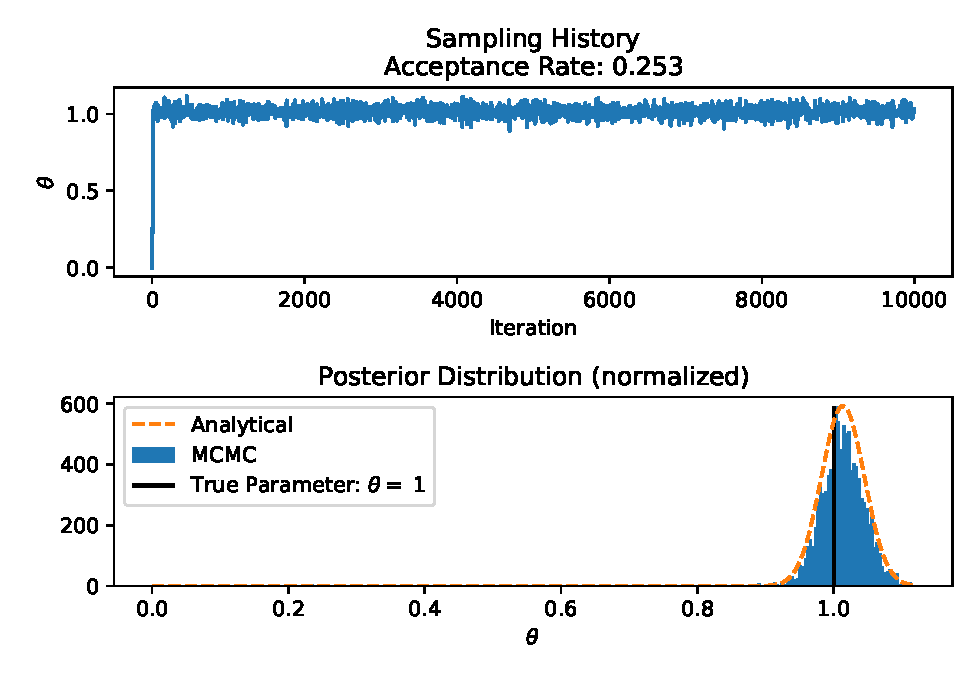
\includegraphics{/Users/macowner/Documents/Stochastic_Calculus/Hmwk_09/hmwk_09_files/figure-latex/metropolis hastings-1.pdf}
\# References

\hypertarget{refs}{}
\leavevmode\hypertarget{ref-sarkka2019applied}{}%
Särkkä, Simo, and Arno Solin. 2019. \emph{Applied Stochastic
Differential Equations}. Vol. 10. Cambridge University Press.


\end{document}
